\documentclass{article}
\usepackage[slovak]{babel}
\usepackage[utf8]{inputenc}

\usepackage{indentfirst}
\usepackage{graphicx}
\usepackage{lscape}

\begin{document}
    \begin{titlepage}
        \begin{center}
            \vspace{\stretch{0.382}}
            
            
\includegraphics[width=10cm]{FITlogo.png}\\[30mm]
            
            \LARGE
            Implementácia prekladača imperatívneho jazyka IFJ17 \\
            \large
            Dokumentácia k~projektu IFJ/IAL\\[55mm]
            
            \begin{tabular}{r l l}
                Tím: & 094 & \\
                Varianta: & II & \\
                Vedúci: & Tomáš Nereča (xnerec00) & 26\% \\
                Ďalší členovia: & Samuel Obuch (xobuch00) & 26\% \\
                    & Jiří Vozár (xvozar04) & 26\% \\
                    & Ján Farský (xfarsk00) & 22\% \\
                Implementované rozšírenia: & BASE, FUNEXP, IFTHEN &\\
            \end{tabular}
            
            \vspace{\stretch{0.618}}
        \end{center}
    \end{titlepage}

    \tableofcontents
    \newpage
    
    \section{Úvod}
        Dokumentácia popisuje implementáciu prekladača imperatívneho jazyka IFJ17. Prekladač načítava
        zdrojový kód jazyka IFJ17 zo~štandardného vstupu a ten pomocou lexikálnej, syntaktickej a sémantickej
        analýzy vyhodnotí a vygeneruje potrebné inštrukcie v~IFJcode17 pre interpret. V~prípade
        výskytu chyby pri analýze kódu IFJ17 prekladač vráti kód príslušnej chyby a chybovú hlášku na štandardný
        chybový výstup.
        
        Dokumentácia taktiež zahŕňa zhodnotenie práce v~tíme a približuje logiku a fungovanie
        jednotlivých častí prekladača. 
    
    \section{Implementácia}
    
        \subsection{Lexikálna analýza}
        
        \subsection{Syntaktická analýza}
            Překladač využívá syntaxí řízený překlad, ve kterém kombinuje \emph{rekurzivní sestup} pro základní konstrukce
            a příkazy jazyka s \emph{precedenční syntaktickou analýzou} pro výrazy.
            Vstupním bodem překladače je funkce \texttt{parse}, která zavolá vyhodnocení hlavního neterminálu \emph{program},
            který po kontrole volá funkce z něho vycházejících dalších neterminálů.
            Pokud pravidlo očekává výraz, je volána funkce \texttt{expression}, která se postará o vyhodnocení výrazu převodem
            do postfixové podoby.
            
            \subsubsection{Rekurzívny zostup}
                Pro každý neterminál je vytvořena funkce, která je volána pro vyhodnocení daného neterminálu.
                Funkce poté vrací hodnotu \texttt{true}, pokud bylo vyhodnocení úspěšné a hodnotu \texttt{false}, pokud došlo k nějaké chybě. Některé funkce z důvodu zjednodušení nereprezentují pravidla úplně přesně, kdy se například funkce \texttt{statementList} nevolá rekurzivně, ale je řízena cyklem. Samotný sestup je rozdělen do 3 modulů pro oddělení obecných neterminálů, neterminálů příkazů a neterminálů funkcí.
            
            \subsubsection{Precedenčná syntaktická analýza}
    
        \subsection{Tabuľka symbolov}
            Tabulka symbolů je implementována jako hash tabulka. Hashovací funkce byla zvolena \emph{djb2}\footnote{\texttt{http://www.cse.yorku.ca/\~{}oz/hash.html}}, jelikož dávala dobré výsledky rozložení při experimentování s větším množstvím záznamů.
            
            Informace o symbolu jsou poté ukládány ve struktuře, která byla navržená univerzálně pro informace o proměnných i funkcích.
        
        \subsection{Vstavané funkcie}
            V prekladači sme implementovali aj štyri vstavané funkcie pre jazyk IFJ17.
            
            \subsubsection{Length}
            Vstupným parametrom funkcie je string a výstupným je číselná hodnota dĺžky vstupného stringu.
            
            \subsubsection{SubStr}
            Vstupné parametre funkcie sú string  a dva integery. Výstupom je podreťazec vstupného
            stringu, ktorého začiatok je určený prvým integerom a jeho dĺžka druhým. Ak je index dĺžky
            0 alebo indexujeme mimo medze stringu návratovou hodnotou je prázdny reťazec. Ak by časť 
            znakov podreťazca pripadala mimo medze základného stringu návratovou hodnotou je string
            obsahujúci iba znaky z~medzí vstupného stringu.
            
            \subsubsection{Asc}
            Vstupné parametre funkcie sú reťazec string a integer. Výstupnou hodnotou je ordinálna
            hodnota (ASCII) znaku v~stringu na pozícii zadanej integerom. Ak integer zasahuje mimo 
            medze stringu návratovou hodnotou je 0.
            
            \subsubsection{Chr}
            Vstupným parametrom je integer. Výstupom je znak, ktorého ASCII kód bol zadaný integerom.
            V~prípade integeru momo medzí 0-255 je chovanie funkcie nedefinované.
            
        \subsection{Generovanie kódu}
            Cílový kód je generován přímo během jediného průchodu vypisováním příslušných instrukcí ve funkci
            příslušného pravidla.
            
            Proměnné definované uživatelem se ukládají na datový rámec, který se pro funkce
            tvoří vždy nový.
            Výrazy využívají pro mezivýsledky zásobník, kam se ukládají i vyhodnocené parametry a výsledky funkcí.
            
            Podmínky a cykly využívají instrukce podmíněných a nepodmíněných skoků, ale funkce se volají instrukcemi \texttt{CALL}
            a \texttt{RETURN}.
        
    \section{Rozšírenia}
    Boli implementované celkom 3 rozšírenia
        \begin{itemize}
            \item \textbf{base}   - podpora zadávania celočíselných konštánt v~2, 8 a 16-tkovej sústave.
            \item \textbf{funexp} - podpora volania funkcií, ktoré môžu v~argumentoch obsahovať výrazy 
                                        a zároveň súčasťou výrazu môže byť volanie funkcie.
            \item  \textbf{ifthen} - podpora zjednodušenej konštrukcie podmienky If-Then bez časti Else
                                        a zároveň viacnásobnej konštrukcie Elseif-Then.
        \end{itemize}
    
    \section{Testovanie}
    Na začiatku sme určili jedného člena, ktorý písal jednotkové testy pre lexikálny analyzátor. 
    Neskôr sme napísali zopár vlastných regresných testov.
    
    Keď sme sa dozvedeli o~verejnej databáze testov našich kolegov. Do nej sme prispeli aj vlastnými testami a využili ostatné testy na čo najrobustnejšie otestovanie funkčnosti nášho prekladača.
    
    \section{Práca v~tíme}
    Ako tím sme sa začali schádzať pomerne skoro po zaregistrovaní nášho zadania. Stretnutie sme mali 
    minimálne raz týždenne, kde sme prediskutovali aktuálny stav práve implementovaných častí 
    a ďalší postup či korekciu v~zdrojovom kóde. Prácu sme sa snažili rozdeľovať rovnomerne medzi 
    všetkých členov tímu čo sa nie vždy darilo. Po pridelení úlohy sme stanovili deadline, aby sme 
    mohli čo najskôr pokračovať na nasledujúcej časti projektu. Jednotlivé časti sme sa snažili 
    implementovať paralelne s~preberanou látkou na prednáškach aby sme korektne implementovali
    jednotlivé časti a vyhli sa zbytočným chybám.

        \subsection{Správa zdrojového kódu}
        Pre správu a zdielanie zdrojových súborov sme využili verzovací systém \emph{Git} a webovú službu GitHub pre vzdialené ukladanie, ktorú sme už 
        počas štúdia využili na verzovanie projektov v~iných predmetoch.
        
        Ako komunikačný kanál sme 
        prevažne využívali skupinovú konverzáciu na sociálnej sieti Facebook, ktorá nám všetkým 
        vyhovovala.
        
        Na sledovanie postupu pri plnení pridelených úloh a oznamovanie nájdených chýb 
        sme využívali online nástroj Trello, ktorý slúži ako online kanban pre sledovanie projektov. 
        
        Vďaka týmto informačným kanálom mohli mať všetci členovia tímu prístup k~najaktuálnejšej
        verzii projektu a reagovať na vzniknuté chyby efektívne.

        \newpage
        \subsection{Rozdelenie}
        \noindent
        Bodové rozdelenie je nasledovné:\\~\\
        \begin{tabular}{l l}
            Tomáš Nereča (xnerec00) & 26\% \\
            Samuel Obuch (xobuch00) & 26\% \\
            Jiří Vozár (xvozar04)   & 26\% \\
            Ján Farský (xfarsk00)   & 22\% \\
        \end{tabular} \\
        Dôvod nerovnomerného rozdelenia bodov bolo nedostatočné splnenie pridelených častí jednému 
        z~členov tímu, čo viedlo k~potrebnému prepisu zdrojového kódu ostatnými členmi tímu.

    \section{Záver}
    S~projektom podobného rozsahu sa ešte nikto z~nás predtým nestretol, preto ho pokladáme za dobrú
    skúsenosť pre každého z~nás. Pri jeho riešení sme prakticky využili získané vedomosti z~predmetov 
    IFJ a IAL.
    
    Pre správne fungovanie tímu bola potrebná dobrá komunikácia, riadenie a pridelovanie úloh, ktoré pretvali počas celého
    priebehu projektu či už vďaka pravidelným stretnutiam alebo využitým nástrojom ale aj individuálne
    schopnosti jednotlivých členov. Výsledkom tejto práce je funkčný a z~nášho pohľadu vydarený 
    prekladač jazyka IFJ17.
    
    \newpage
    \section{Prílohy}
        \subsection{Diagram konečného automatu}
            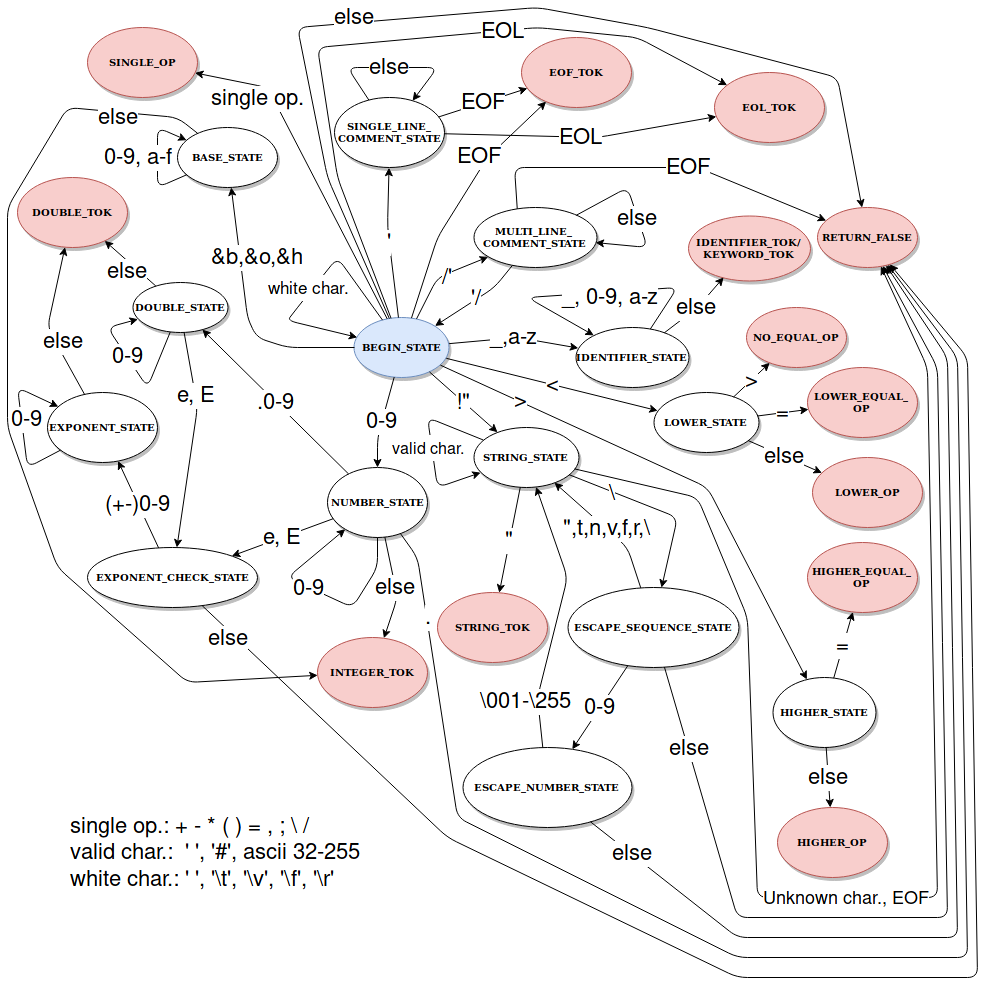
\includegraphics[trim=6cm 0 0 0, width=15cm]{finite_automata.png}
            \newpage
            
        \subsection{LL gramatika}
            \begin{enumerate}
                % NESAHAT - zhenodnotí čísla v tabulce LL gramatiky!
                \item \texttt{<program> -> declare function <functionDecl> eol <program>}
                \item \texttt{<program> -> function <functionDef> eol <program>}
                \item \texttt{<program> -> scope <statementList> end scope}
                
                \item \texttt{<functionDecl> -> <functionHeader>}
                \item \texttt{<functionDef> -> <functionHeader> eol <statementList> end function}
                
                \item \texttt{<functionHeader> -> identifier ( <functionParams> ) as type}
                
                \item \texttt{<functionParams> -> <functionParam> <nextFuncParam>}
                \item \texttt{<functionParams> -> epsilon}
                
                \item \texttt{<nextFuncParam> -> , <functionParam> <nextFuncParam>}
                \item \texttt{<nextFuncParam> -> epsilon}
                
                \item \texttt{<functionParam> -> identifier as type}
                
                \item \texttt{<statementList> -> <statement> eol <statementList>}
                \item \texttt{<statementList> -> epsilon}
                
                \item \texttt{<statement> -> dim <declaration>}
                \item \texttt{<statement> -> identifier = <expression>}
                \item \texttt{<statement> -> input identifier}
                \item \texttt{<statement> -> print <printArgs>}
                \item \texttt{<statement> -> if <expression> then eol <statementList> <else>}
                \item \texttt{<statement> -> do while <expression> eol <statementList> loop}
                \item \texttt{<statement> -> return identifier}
                
                \item \texttt{<declaration> -> identifier as type}
                \item \texttt{<declaration> -> identifier as type = <expression>}
                
                \item \texttt{<printArgs> -> <expression> ;}
                \item \texttt{<printArgs> -> <expression> ; <printArgs>}
                
                \item \texttt{<else> -> elseif <expression> then eol <else> end if}
                \item \texttt{<else> -> else eol <statementList> end if}
                \item \texttt{<else> -> end if}
                
                \item \texttt{<expression> ->} vyhodnocuje se precedenční syntaktickou analýzou
            \end{enumerate}
        \newpage
        
        \subsection{LL tabuľka}
        \newcommand{\tterm}[1]{\rotatebox[origin=c]{90}{\texttt{#1}}}
            \begin{tabular}{|r|*{10}{c|}}
                \hline
                & \tterm{declare} & \tterm{function} & \tterm{scope} & \tterm{identifier} & \tterm{dim} &
                \tterm{input} & \tterm{print} & \tterm{if} & \tterm{do} & \tterm{return} \\\hline \hline
                \texttt{<program>} & 1 & 2 & 3 &&&&&&& \\\hline
                \texttt{<functionDecl>} &&&& 4 &&&&&& \\\hline
                \texttt{<functionDef>} &&&& 5 &&&&&& \\\hline
                \texttt{<functionHeader>} &&&& 6 &&&&&& \\\hline
                \texttt{<functionParams>} &&&& 7, 8 &&&&&& \\\hline
                \texttt{<nextFuncParam>} &&&&&&&&&& \\\hline
                \texttt{<functionParam>} &&&& 11 &&&&&& \\\hline
                \texttt{<statementList>} &&&& 12 & 12 & 12 & 12 & 12 & 12 & 12 \\\hline
                \texttt{<statement>} &&&& 15 & 14 & 16 & 17 & 18 & 19 & 20 \\\hline
                \texttt{<declaration>} &&&& 21, 22&&&&&& \\\hline
                \texttt{<else>} &&&& 23, 24&&&&&& \\\hline
            \end{tabular}
            
            \begin{tabular}{|r|*{9}{c|}}
                \hline
                & \tterm{elseif} & \tterm{else} & \tterm{end} & \tterm{loop} & \tterm{eol} &
                \tterm{(} & \tterm{)} & \tterm{=} & \tterm{,} \\\hline \hline
                \texttt{<program>} &&&&&&&&& \\\hline
                \texttt{<functionDecl>} &&&&&&&&& \\\hline
                \texttt{<functionDef>} &&&&&&&&& \\\hline
                \texttt{<functionHeader>} &&&&&&&&& \\\hline
                \texttt{<functionParams>} &&&&&&& 8 && \\\hline
                \texttt{<nextFuncParam>} &&&&&&& 10 && 9 \\\hline
                \texttt{<statementList>} & 13 & 13 & 13 & 13 &&&&& \\\hline
                \texttt{<statement>} &&&&&&&&& \\\hline
                \texttt{<declaration>} &&&&&& 23, 24&&& \\\hline
                \texttt{<else>} & 25 & 26 & 27 &&&&&& \\\hline
            \end{tabular}
        \newpage

        \subsection{Precedenčná tabuľka}

\end{document}